\PassOptionsToPackage{unicode=true}{hyperref} % options for packages loaded elsewhere
\PassOptionsToPackage{hyphens}{url}
%
\documentclass[a4paper, xcolor = usenames,dvipsnames]{article}
\usepackage{lmodern}
\usepackage{amssymb,amsmath}
\usepackage{ifxetex,ifluatex}
\usepackage{fixltx2e} % provides \textsubscript
\ifnum 0\ifxetex 1\fi\ifluatex 1\fi=0 % if pdftex
  \usepackage[T1]{fontenc}
  \usepackage[utf8]{inputenc}
  \usepackage{textcomp} % provides euro and other symbols
\else % if luatex or xelatex
  \usepackage{unicode-math}
  \defaultfontfeatures{Ligatures=TeX,Scale=MatchLowercase}
\fi
% use upquote if available, for straight quotes in verbatim environments
\IfFileExists{upquote.sty}{\usepackage{upquote}}{}
% use microtype if available
\IfFileExists{microtype.sty}{%
\usepackage[]{microtype}
\UseMicrotypeSet[protrusion]{basicmath} % disable protrusion for tt fonts
}{}
\IfFileExists{parskip.sty}{%
\usepackage{parskip}
}{% else
\setlength{\parindent}{0pt}
\setlength{\parskip}{6pt plus 2pt minus 1pt}
}
\usepackage{hyperref}
\hypersetup{
            pdftitle={Digital simulation of the movement of an atlatl},
            pdfauthor={Μapia; VO Van Nghia; PHAM Tuan Kiet},
            pdfborder={0 0 0},
            breaklinks=true}
\urlstyle{same}  % don't use monospace font for urls
\usepackage[margin=2.5cm]{geometry}
\usepackage{listings}
\newcommand{\passthrough}[1]{#1}
\usepackage{longtable,booktabs}
% Fix footnotes in tables (requires footnote package)
\IfFileExists{footnote.sty}{\usepackage{footnote}\makesavenoteenv{longtable}}{}
\usepackage{graphicx,grffile}
\makeatletter
\def\maxwidth{\ifdim\Gin@nat@width>\linewidth\linewidth\else\Gin@nat@width\fi}
\def\maxheight{\ifdim\Gin@nat@height>\textheight\textheight\else\Gin@nat@height\fi}
\makeatother
% Scale images if necessary, so that they will not overflow the page
% margins by default, and it is still possible to overwrite the defaults
% using explicit options in \includegraphics[width, height, ...]{}
\setkeys{Gin}{width=\maxwidth,height=\maxheight,keepaspectratio}
\setlength{\emergencystretch}{3em}  % prevent overfull lines
\providecommand{\tightlist}{%
  \setlength{\itemsep}{0pt}\setlength{\parskip}{0pt}}
\setcounter{secnumdepth}{5}
% Redefines (sub)paragraphs to behave more like sections
\ifx\paragraph\undefined\else
\let\oldparagraph\paragraph
\renewcommand{\paragraph}[1]{\oldparagraph{#1}\mbox{}}
\fi
\ifx\subparagraph\undefined\else
\let\oldsubparagraph\subparagraph
\renewcommand{\subparagraph}[1]{\oldsubparagraph{#1}\mbox{}}
\fi

% set default figure placement to htbp
\makeatletter
\def\fps@figure{htbp}
\makeatother

\usepackage{setspace}
\usepackage{float}
\usepackage{fontspec}
\usepackage{subfig}
\usepackage{hyperref}
\usepackage{mathtools}
\usepackage{gensymb}
\floatplacement{figure}{H}
\lstset{
  language=C,
  basicstyle={\linespread{0.8}\ttfamily},
  stepnumber=1,
  numbersep=5pt,
  backgroundcolor=\color{cyan!5},
  showspaces=false,
  showstringspaces=false,
  showtabs=false,
  frame=single,
  rulecolor=\color{black},
  tabsize=2,
  captionpos=b,
  breaklines=true,
  breakatwhitespace=false,
  keywordstyle=\color{RoyalBlue},
  commentstyle=\color{Green},
  stringstyle=\color{Orange},
  keepspaces=true
}
\makeatletter
\renewcommand\paragraph{\@startsection{paragraph}{4}{\z@}%
  {-2.5ex\@plus -1ex \@minus -.25ex}%
  {1.25ex \@plus .25ex}%
  {\normalfont\normalsize\bfseries}}
\makeatother
\setcounter{secnumdepth}{4}
\hypersetup{
  colorlinks = true,
}
\usepackage[]{biblatex}
\addbibresource{ref.bib}

\title{Digital simulation of the movement of an atlatl}
\author{Μapia \and VO Van Nghia \and PHAM Tuan Kiet}
\date{}

\begin{document}
\maketitle
\begin{abstract}
One of the special weapons rarely seen nowadays in television or newspapers is the atlatl, or simply a spear-thrower. Developed in Europe over 30 000 years ago and by the Native North-Americans tribes 12 000 years ago, the atlatl is the first true ``weapon system'' consisting of a projectile (the dart) and a launching device (the atlatl).

The project aims to simulate and optimize the throwing action using a robotic approach. More specifically, we illustrate the movement using Python with the help of Pinocchio. The robot model will consist only of the upper body, which includes the hip, the shoulder, the elbow, and the wrist, in 2D, where only the rotation joint is used.

The work starts with designing a stick-version of the upper body and calculating the distance, the angle of each articulation, creating a ``realistic'' 2D-version of the throwing action, and finally optimizing it for the longest throwing distance of the projectile. From this project, we hope to have a better simulation of the action of throwing atlatl with the dynamic relation to have further studies about this kind of weapon.
\end{abstract}

\hypertarget{introduction}{%
\section{Introduction}\label{introduction}}

Maria (Historical evidences)

\hypertarget{preliminary}{%
\section{Preliminary}\label{preliminary}}

In the first section, we introduce some general notions and theories that we used for modeling a movement of a robot.

\hypertarget{trajectory-planning}{%
\subsection{Trajectory planning}\label{trajectory-planning}}

\hypertarget{from-human-to-robot}{%
\subsubsection{From human to robot}\label{from-human-to-robot}}

The movement of a robot is captured as a series of positions, or a trajectory. For example, the modeling of a walking human is shown below.

\begin{figure}

{\centering 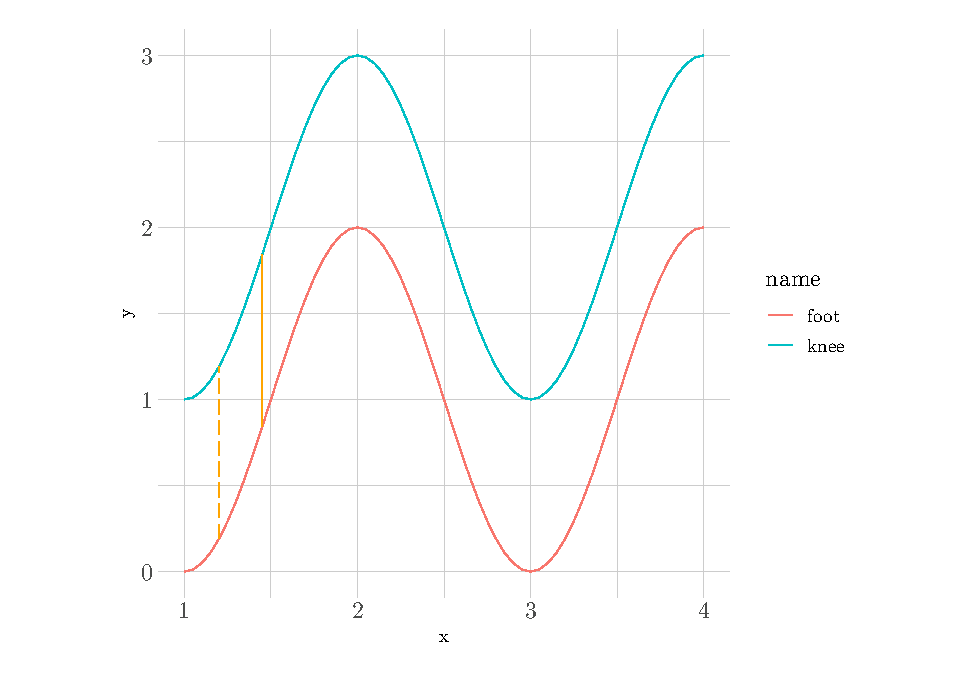
\includegraphics{report_files/figure-latex/human-plot-1} 

}

\caption{Knee and foot trajectory while walking}\label{fig:human-plot}
\end{figure}

There are two curves, each represents a trajectory of our knee and foot while walking. For a better illustration, we also include an orange line which represents the leg. We could imagine a robot that is walking along the \(x\)-axis. With these trajectories, the knee and the foot of the robot will produce a human-like walking movement.

\hypertarget{trajectory-interpolation}{%
\subsubsection{Trajectory interpolation}\label{trajectory-interpolation}}

In the above example, the trajectory could be expressed as a variation of the \(cos\) function. However, in reality, the desired trajectory is more complicated. Computing directly that function is not possible. Instead of doing that, we will only supply some positions at certain times, and interpolate the whole trajectory. To ensure a correct movement, two conditions must be satisfied:

\begin{itemize}
\tightlist
\item
  The interpolator must be smooth. Mathematically, we want the interpolator line is continous and its first derivate is also continouse. This ensures that our robot will not perform any change in action too harshly.
\item
  The monocity of the dataset (positions) being interpolated must be preserved. This keeps the interpolator from generating data that is out of range. (e.g the position of a foot is always greater or equal to \(0\)).
\end{itemize}

For clarity, we will illustrate these 2 conditions below.

\begin{figure}

{\centering 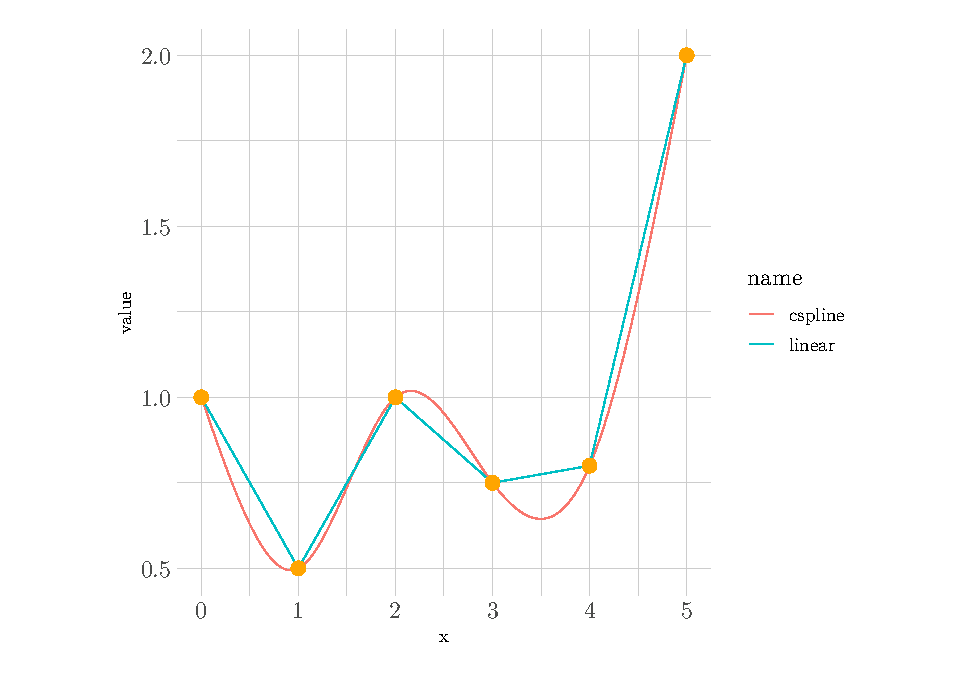
\includegraphics{report_files/figure-latex/smooth-plot-1} 

}

\caption{Smoothness of linear and cubic spline interpolation method}\label{fig:smooth-plot}
\end{figure}

As in figure \ref{fig:smooth-plot}, the linear method only uses straight lines to connect the points together and has a zigzag pattern. On the other side, the cubic spline method is smooth and derivable. Since the graph of each function is also how our robot move its leg, we prefer the cubic spline method for a smooth movement.

\begin{figure}

{\centering 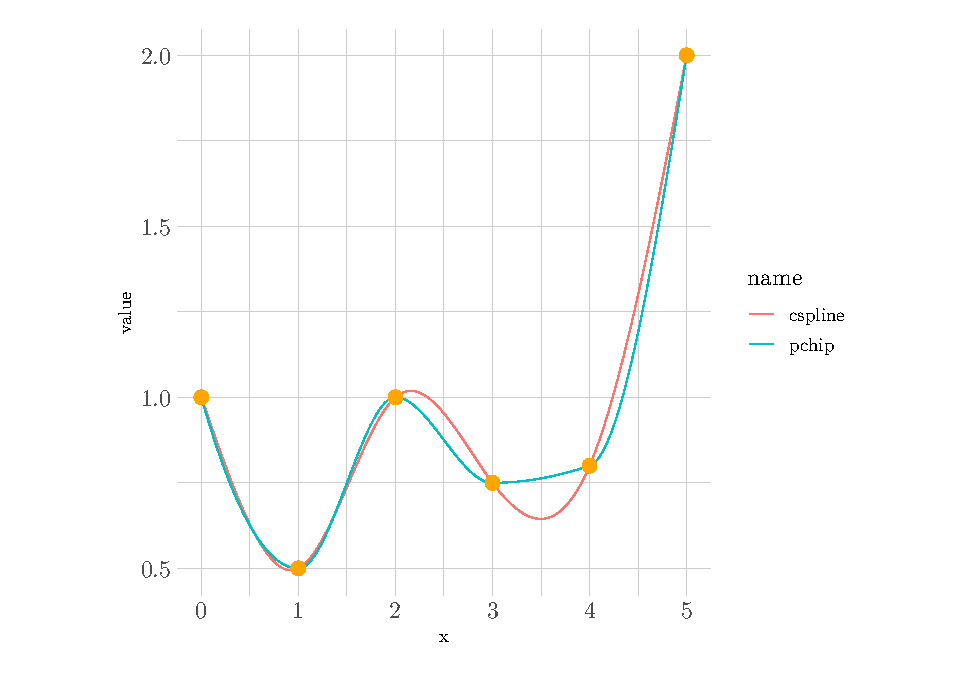
\includegraphics{report_files/figure-latex/mono-plot-1} 

}

\caption{Monocity of cubic spline and pchip interpolation method}\label{fig:mono-plot}
\end{figure}

For the second condition, the figure \ref{fig:mono-plot} shows clearly that the cubic spline method does not respect the monocity between each pair of points while the pchip method (stands for Piecewise Cubic Hermite Interpolating Polynomial) does. For example, if we consider the interval between \(3\) and \(4\), we see that the pchip line is monotonically increasing while the cubic spline forms a valley.

The method that satisfy both conditions is PCHIP\footnote{\url{https://en.wikipedia.org/wiki/Monotone_cubic_interpolation}} and will be used for modeling our robot.

\hypertarget{configuration-solver}{%
\subsection{Configuration solver}\label{configuration-solver}}

A configuration \(q\) is a collection of parameters of a robot and the angle as well as position of each joint of our robot is tied to one unique configuration. We note that \(\mathbb{Q}\) is the set of all configurations (configuration space) of each robot, \(\mathbb{P}\) is the set of all positions of that robot. In addition, \(f: \mathbb{Q} \rightarrow \mathbb{P}\) maps each configuration with its corresponding position, we have \(f\) is bijective. Given a trajectory \(T\), we want to solve the problem below:

\begin{equation}
  \text{ For each } t \text{, find } q \in \mathbb{Q} \text{ such that } f(q) = T(t) \label{eq:config-analy}
\end{equation}

Solving \eqref{eq:config-analy} analytically is generally impossible. Therefore, we transform it to a different optimization problem:

\begin{equation}
  \text{ For each } t \text{, note } q_{t}^{*} \text{ the solution of } \eqref{eq:config-analy} \text{, find } q \in \mathbb{Q} \text{ such that } \| f(q_{t}^{*}) - f(q) \| \text{ is minimized} \label{eq:config-optim}
\end{equation}

Solving \eqref{eq:config-optim} is equivalent to find a close approximation of \(q_{t}^{*}\). We now only need to define the norm \(\| \cdot \|\). Since the position of a robot is specified by the rotation and translation of its components and we might only need to control certain rotations and translations, given \(\{p_{1}^{*}, \dots, p_{n}^{*}\}\) the desired positions at time \(t\) (either rotations and translations), we define the norm as follow:

\[
\| f(q_{t}^{*}) - f(q) \| \coloneqq \sqrt{\sum_{i=1}^{n} (p_{i}^{*} - p_{i})^{2}}
\]

As we do not know the analytical form of \(f\) or neither its gradient, we will use BFGS algorithm\footnote{\url{https://en.wikipedia.org/wiki/Broyden–Fletcher–Goldfarb–Shanno_algorithm}} to solve \eqref{eq:config-optim}.

\hypertarget{directed-angle}{%
\subsection{Directed angle}\label{directed-angle}}

In order to express the translation and rotation easier, we also use directed geometry where anticlockwise angle (\(\theta_{+}\)) are positive and the reference line is the vertical axis of the current frame.

\begin{figure}

{\centering 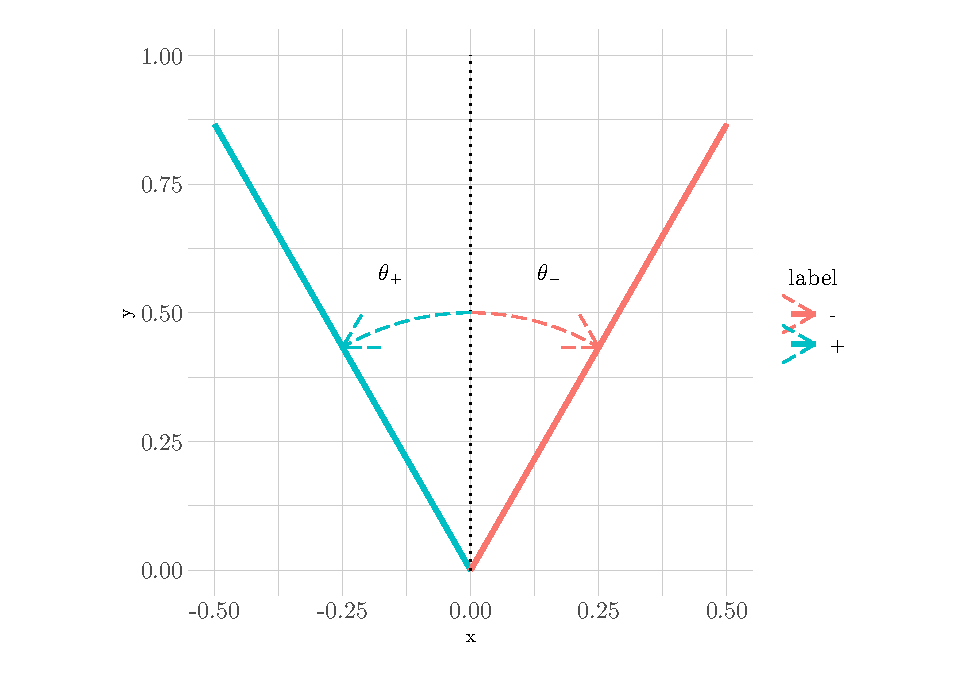
\includegraphics{report_files/figure-latex/angle-plot-1} 

}

\caption{Directed angle}\label{fig:angle-plot}
\end{figure}

\hypertarget{modeling}{%
\section{Modeling}\label{modeling}}

In the second section, we apply previous observations and notions to our problem.

\hypertarget{robot-structure}{%
\subsection{Robot structure}\label{robot-structure}}

First, the structure of our robot is shown below.

\begin{figure}

{\centering 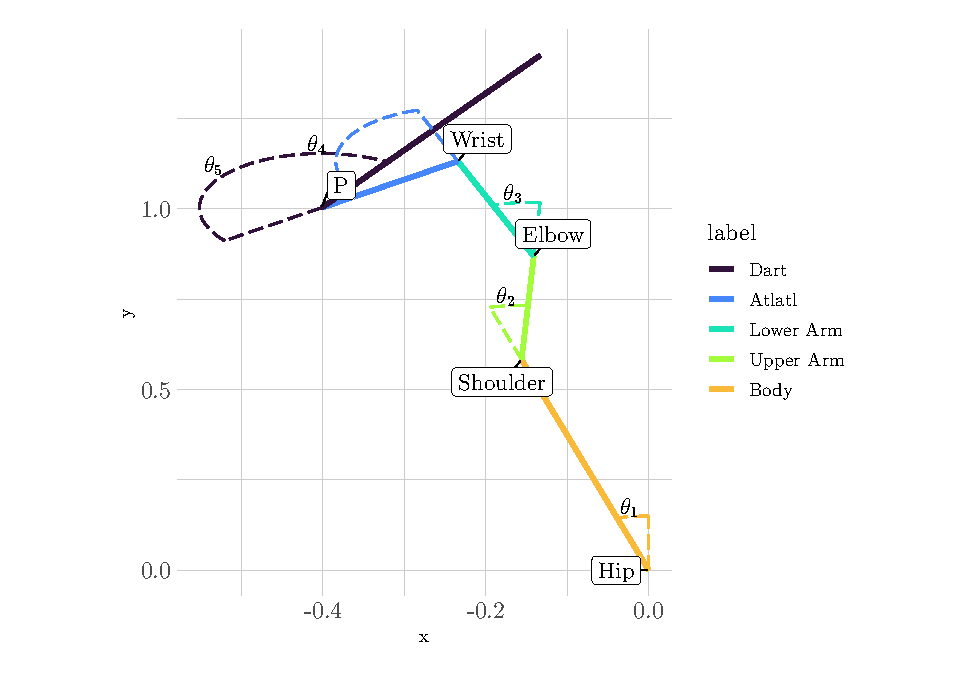
\includegraphics{report_files/figure-latex/initial-model-plot-1} 

}

\caption{Structure of throwing robot}\label{fig:initial-model-plot}
\end{figure}

This structure models our upper body while throwing the atlatl. We have \(5\) rotation joints whose value are \(\theta_{i}\) for \(i \in \{1, 2, 3, 4, 5\}\).

\hypertarget{real-life-observations}{%
\subsection{Real life observations}\label{real-life-observations}}

In order to plan the trajectory of the robot, it is required to study the movement of an atlatl thrower in real life. The movement in real life can be divided into some stages; we first care about the position of the arm and the body, then the one of the wrist and finally, finishing the movement.

\hypertarget{arm-and-body}{%
\subsubsection{Arm and body}\label{arm-and-body}}

The core starts to rotate while the upper arm starts to flex at the height of the shoulder. In this way, the hand and the atlatl are moving until they are almost behind the head. The atlatl throughout this remains horizontal. The shoulder flex seems to be small at this point and the wrist must be rotated to keep the dart pointed at the target.

\begin{figure}

{\centering 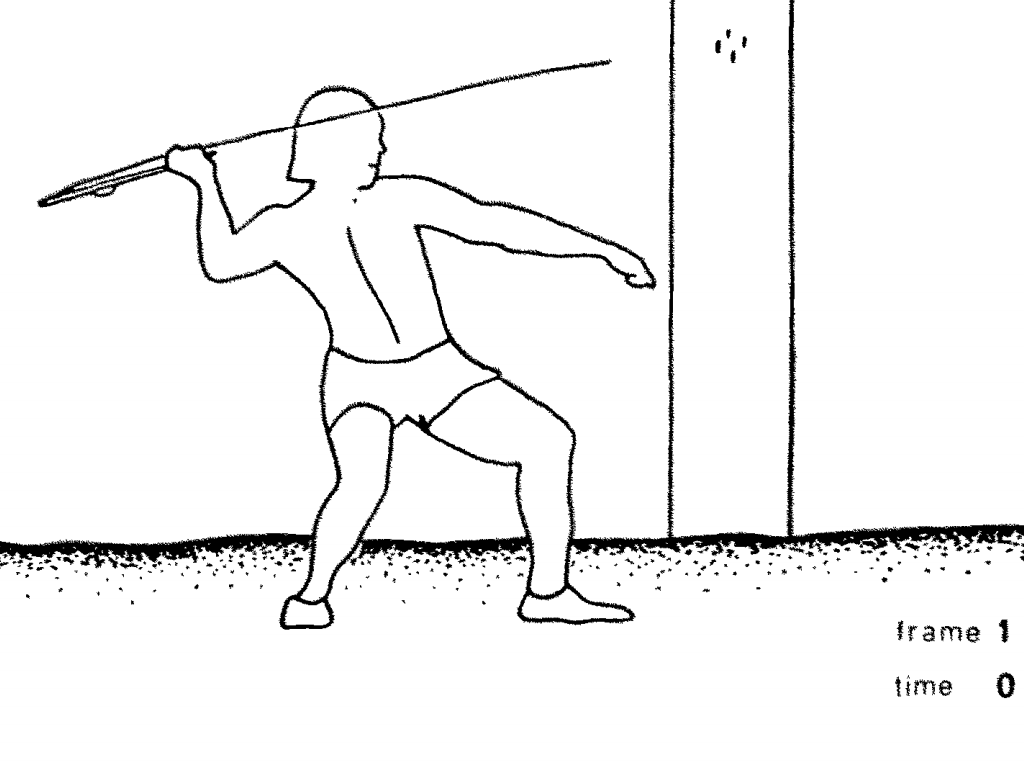
\includegraphics[width=0.3\linewidth]{res/observations/1} 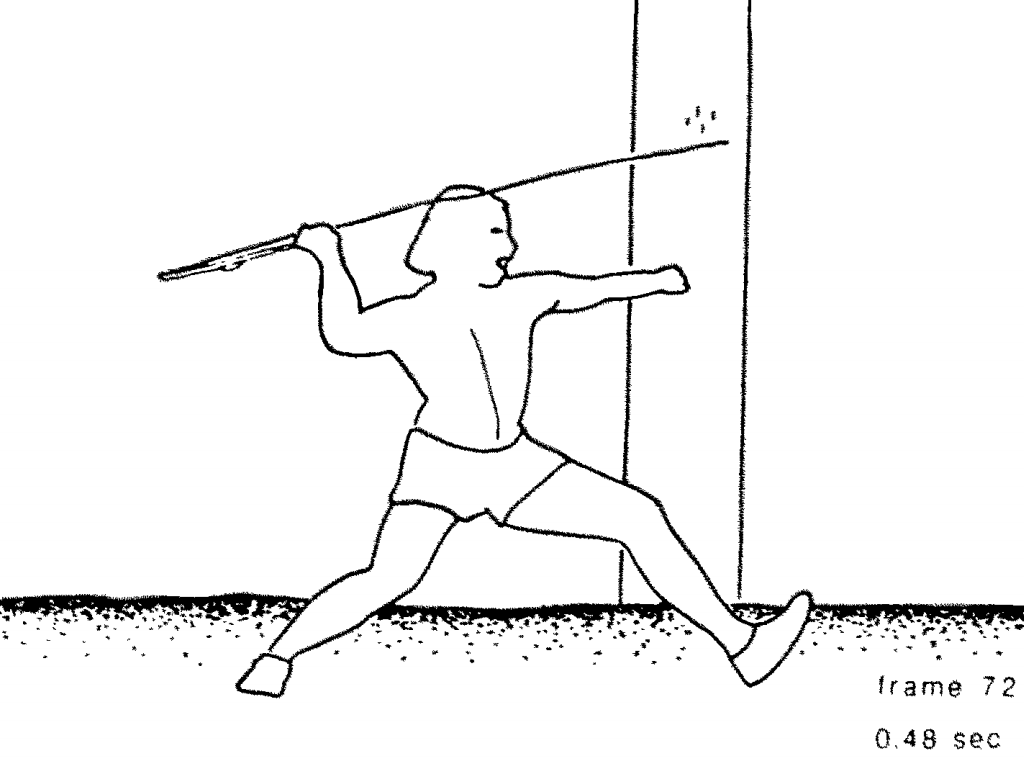
\includegraphics[width=0.3\linewidth]{res/observations/2} 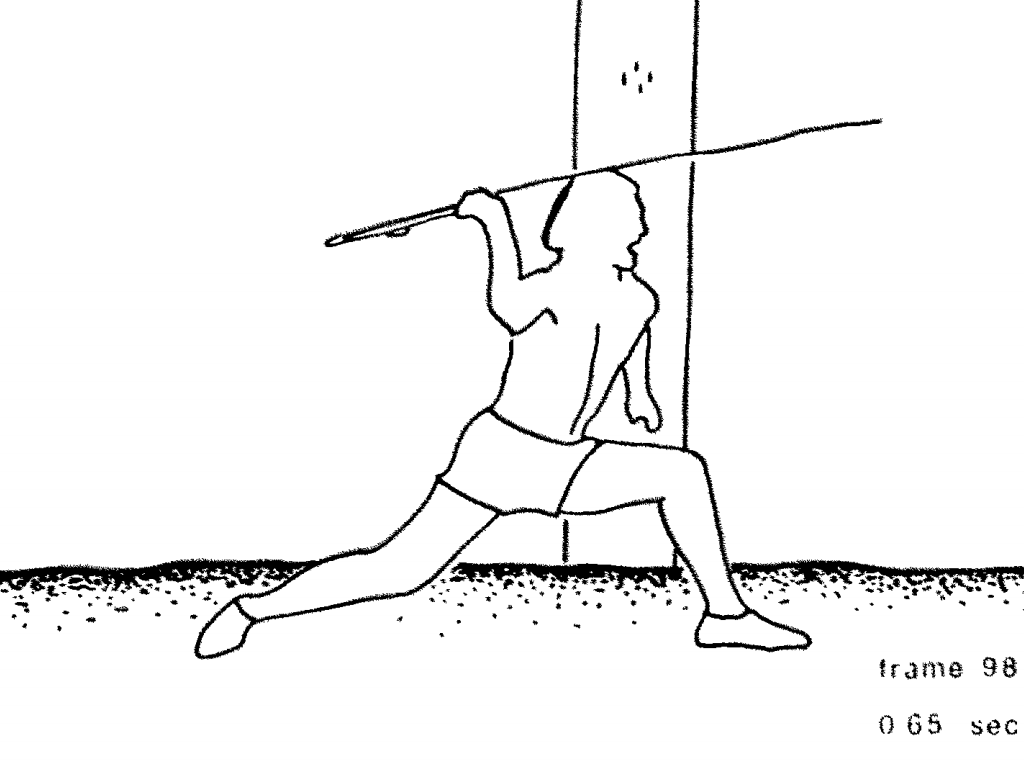
\includegraphics[width=0.3\linewidth]{res/observations/3} 

}

\caption{Position of arm and body}\label{fig:arm-body-pos}
\end{figure}

\hypertarget{wrist}{%
\subsubsection{Wrist}\label{wrist}}

Slightly before the hand reaches the back of the head, the hand and forearm begin to rise. Then as the hand is passing the head, the wrist should snap vigorously, giving the atlatl a vertical position and flicking the dart away. The dart will flex as the point remains aimed to the target, following a straight path. At the same time, the arm is being flexed straight out.

\begin{figure}

{\centering 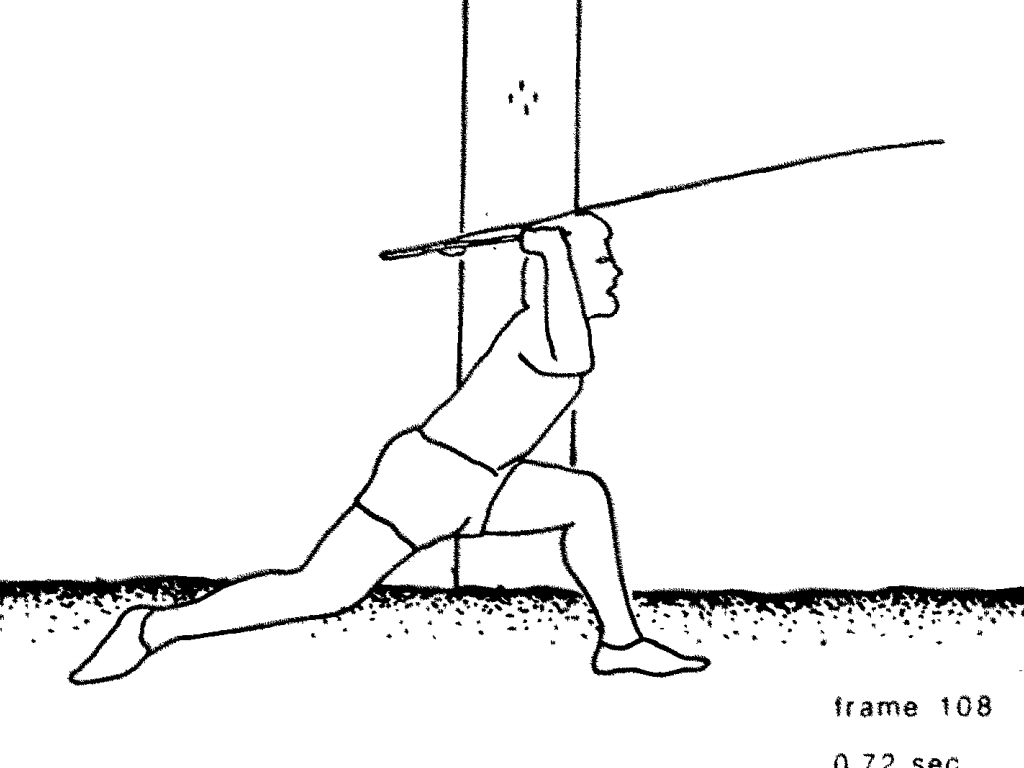
\includegraphics[width=0.3\linewidth]{res/observations/4} 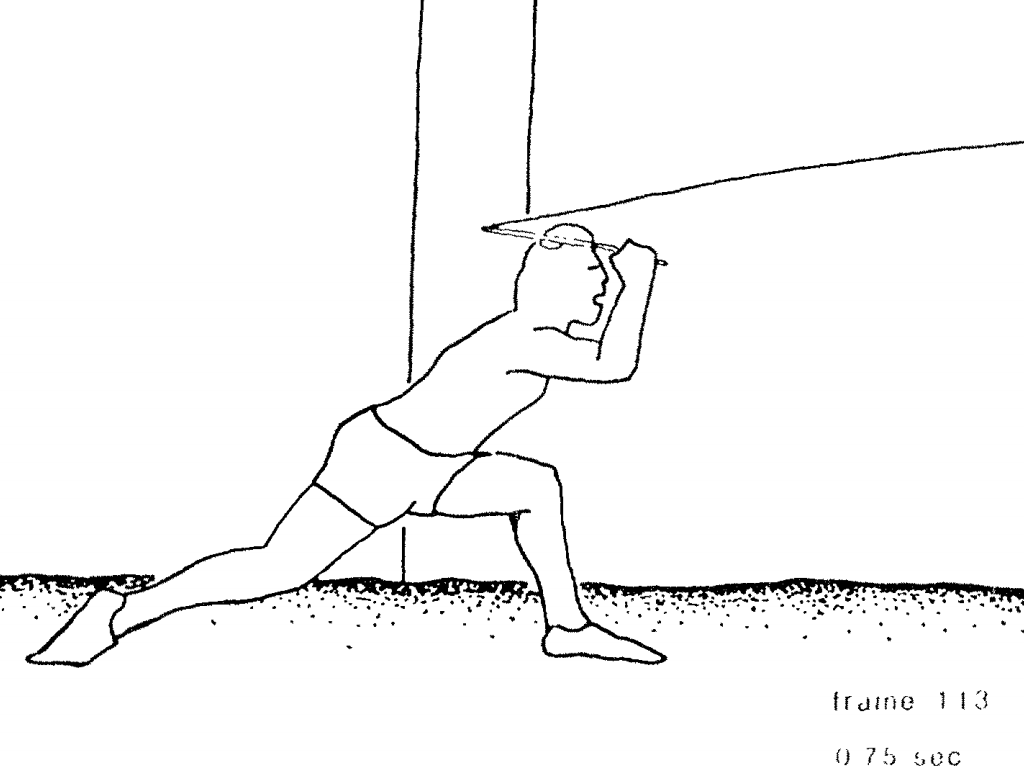
\includegraphics[width=0.3\linewidth]{res/observations/5} 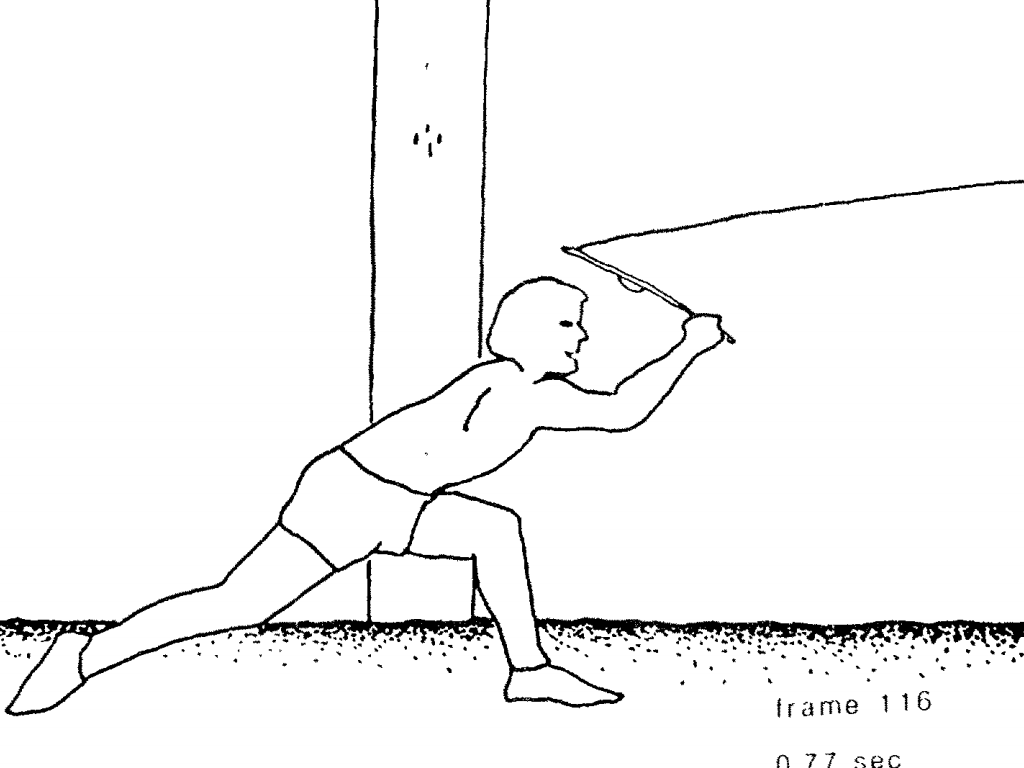
\includegraphics[width=0.3\linewidth]{res/observations/6} 

}

\caption{Position of wrist}\label{fig:wrist-pos}
\end{figure}

\hypertarget{finishing}{%
\subsubsection{Finishing}\label{finishing}}

The dart is higher enough compared to the head when it is just about to leave the atlatl. The vertical position of the atlatl permits the dart to fly away. As the dart is leaving the atlatl, the thrower is leaning slightly forward. The movement finishes in a position where the arm that holds the atlatl crosses the opposite leg.

\begin{figure}

{\centering 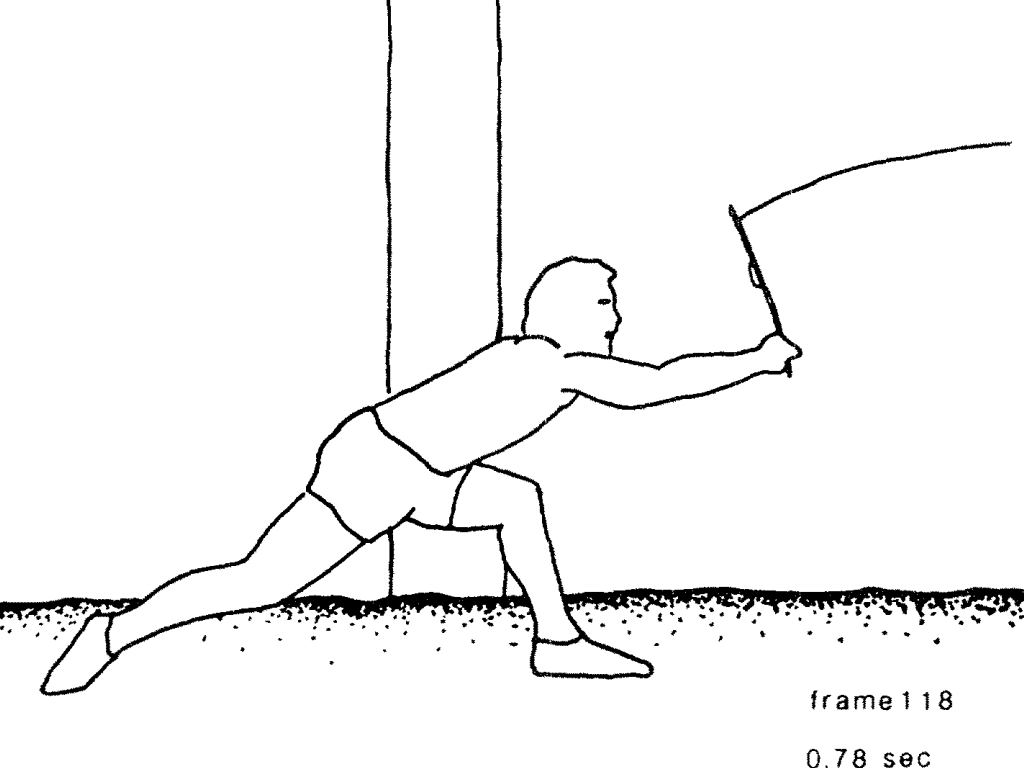
\includegraphics[width=0.3\linewidth]{res/observations/7} 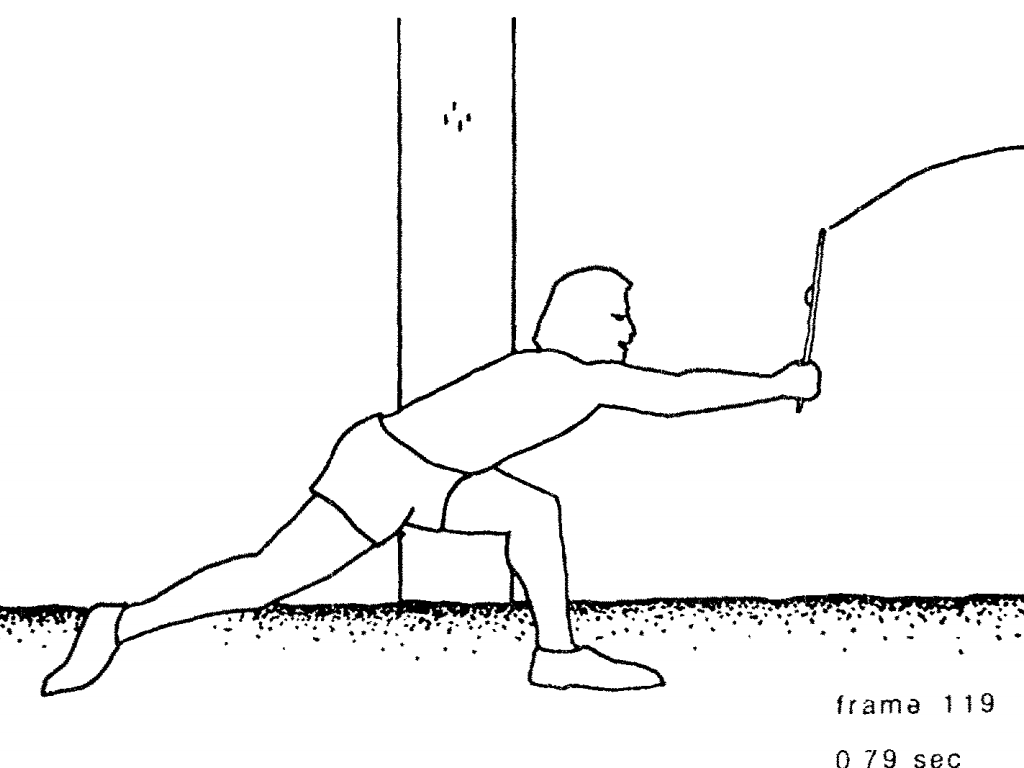
\includegraphics[width=0.3\linewidth]{res/observations/8} 

}

\caption{Finish position}\label{fig:finish-pos}
\end{figure}

\hypertarget{the-atlatl-and-the-dart}{%
\subsubsection{The atlatl and the dart}\label{the-atlatl-and-the-dart}}

Concerning the movement of the atlatl-dart system, \textcite{10.2307/279223} states that when throwing a spear with the unaided hand it is necessary to make the hand travel in a straight line until the spear is released. When the hand nears its maximum outstretched position, the spear is then released. This allows to maintain control of the spear's line and avoid any downward motion. The same thing holds true for a dart that is thrown with the atlatl. Therefore, in addition to these observations above, we also impose another constraint: the distance between P and the ground is constant or the point P moves along a straight line.

\begin{figure}

{\centering 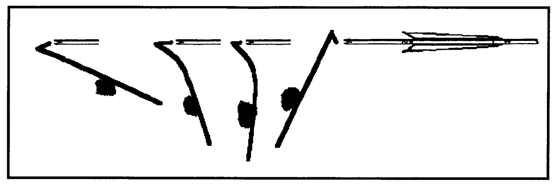
\includegraphics[width=0.75\linewidth]{res/observations/straight} 

}

\caption{Atlatl straight line}\label{fig:constant-P}
\end{figure}

\hypertarget{trajectory-planning-1}{%
\subsection{Trajectory planning}\label{trajectory-planning-1}}

\hypertarget{hip-shoulder-and-elbow}{%
\subsubsection{Hip, shoulder and elbow}\label{hip-shoulder-and-elbow}}

From the observations above, we first supply the rotations value of the first \(3\) joints: hip, shoulder and elbow to the interpolator and obtain the trajectory below:

\begin{figure}

{\centering 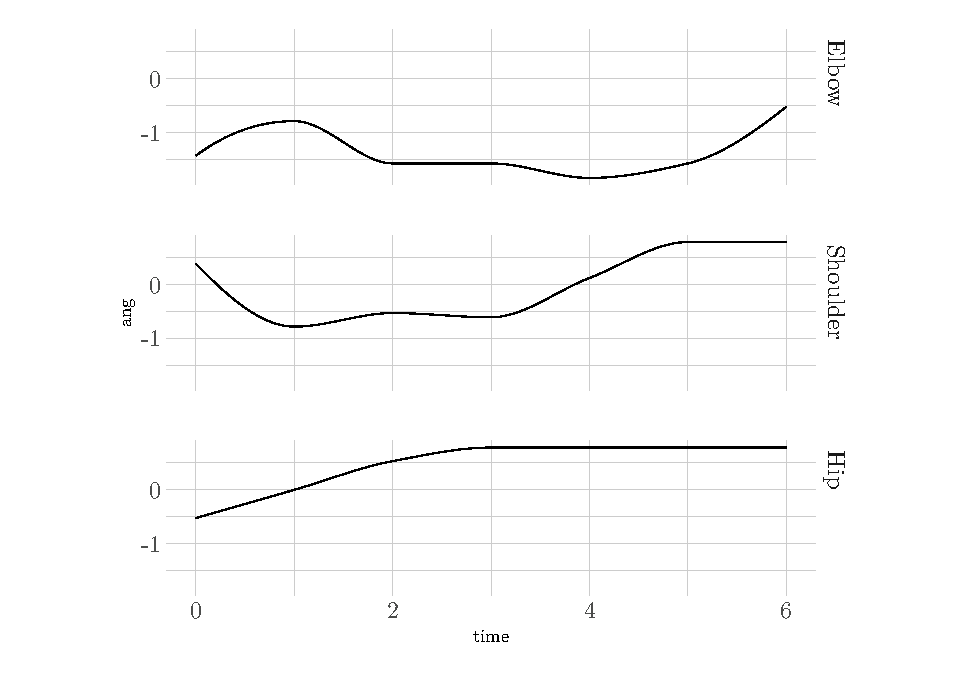
\includegraphics{report_files/figure-latex/traject-hse-plot-1} 

}

\caption{Trajectory of hip, shoulder and elbow}\label{fig:traject-hse-plot}
\end{figure}

\hypertarget{wrist-1}{%
\subsubsection{Wrist}\label{wrist-1}}

For the wrist joint, we want to ensure the constant height as in the previous \protect\hyperlink{the-atlatl-and-the-dart}{section}. If we note \(\theta_{i}\) the angle with respect to the local frame (as in figure \ref{fig:initial-model-plot}), \(\Theta_{i}\) the angle with respect to the root frame, \(l_{i}\) the length of the \(i^{th}\) joint / part respectively and \(h_{i}\) the distance between the \(i^{th}\) joint and ground, we have the following relation:

\begin{equation}
  h_{k} = \sum_{i = 1}^{k} l_{i} cos(\Theta_{i}) \text{ where } \Theta_{j} = \sum_{i = 1}^{j} \theta_{i} \label{eq:wrist}
\end{equation}

From \eqref{eq:wrist}, we can easily calculate \(\theta_4\) as we already know \(h_4\). Below is the trajectory of the wrist joint.

\begin{figure}

{\centering 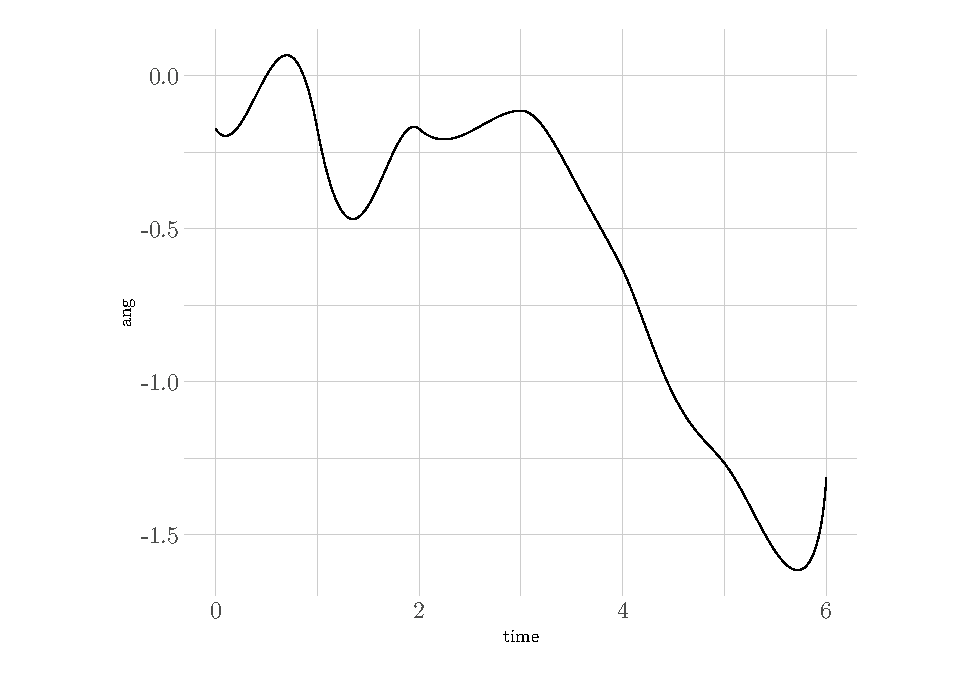
\includegraphics{report_files/figure-latex/traject-wrist-plot-1} 

}

\caption{Trajectory of the wrist joint}\label{fig:traject-wrist-plot}
\end{figure}

\hypertarget{p}{%
\subsubsection{P}\label{p}}

Pham Tuan Kiet

\hypertarget{result}{%
\subsection{Result}\label{result}}

Vo Van Nghia \& Pham Tuan Kiet

\hypertarget{improvement}{%
\section{Improvement}\label{improvement}}

Vo Van Nghia \& Pham Tuan Kiet

\hypertarget{conclusion}{%
\section{Conclusion}\label{conclusion}}

Vo Van Nghia \& Pham Tuan Kiet

\newpage

\printbibliography[title=References]

\end{document}
